%-----------------------------------------------------------------------------
%
%               Template for sigplanconf LaTeX Class
%
% Name:         sigplanconf-template.tex
%
% Purpose:      A template for sigplanconf.cls, which is a LaTeX 2e class
%               file for SIGPLAN conference proceedings.
%
% Author:       Paul C. Anagnostopoulos
%               Windfall Software
%               978 371-2316
%               paul@windfall.com
%
% Created:      15 February 2005
%
%-----------------------------------------------------------------------------


%\documentclass[]{sigplanconf}

% The following \documentclass options may be useful:
%
% 10pt          To set in 10-point type instead of 9-point.
% 11pt          To set in 11-point type instead of 9-point.
% authoryear    To obtain author/year citation style instead of numeric.

%\usepackage{amsmath}
%\usepackage{graphicx}
%\usepackage{url} 


\newcommand{\codesize}{\fontsize{7}{8}\selectfont}

%\begin{document}
%\conferenceinfo{DAMP'12,} {January 28, 2012, Philadelphia, PA, USA.}
%\CopyrightYear{2012}
%\copyrightdata{978-1-4503-1117-5/12/01} 

%\conferenceinfo{WXYZ '05}{date, City.} 
%\copyrightyear{2005} 
%\copyrightdata{[to be supplied]} 

%\titlebanner{}        % These are ignored unless
%\preprintfooter{}   % 'preprint' option specified.

%\title{Towards an Implementation of Push Arrays in Obsidian}
%\title{Expressive Array Constructs in an Embedded GPU Kernel Programming Language}
%\subtitle{Subtitle Text, if any}

%\authorinfo{Name1}
%           {Affiliation1}
%           {Email1}
%\authorinfo{Koen Claessen \and Mary Sheeran \and Bo Joel Svensson}
%           {Chalmers University of Technology, 
%             Department of Computer Science and Engineering,
%             Gothenburg, Sweden}
%           {koen@chalmers.se/ms@chalmers.se/joels@chalmers.se}

%\maketitle

% ABSTRACT !!! -----------------------------------------------------------------
%\begin{abstract}
%This is the text of the abstract.


\subsection*{Abstract}
Graphics Processing Units (GPUs) are powerful computing devices 
that with the advent of CUDA/OpenCL are becomming useful for general 
purpose computations. 
Obsidian is an embedded domain specific language that generates CUDA kernels
from functional descriptions.
A symbolic array construction allows us to guarantee that intermediate
arrays are fused away. However, the current array construction has
some drawbacks; in particular, arrays cannot be combined efficiently.
We add a new type of {\em push arrays} to the existing Obsidian system in 
order to solve this problem. The two array types complement each other,
and enable the definition of combinators that both
take apart and combine arrays, and that result in efficient generated code.
This extension to Obsidian is demonstrated on a sequence of
sorting kernels, with good results.
The case study also illustrates the use of combinators for expressing
the structure of parallel algorithms.
The work presented is preliminary, and 
the combinators presented must be generalised.
However, the raw speed of the generated kernels bodes well.
%\end{abstract}



%\category{CR-number}{subcategory}{third-level}
%\category{D.3.2}{Programming Languages}{Language Classifications}[Applicative (functional) languages; Concurrent, distributed, and parallel languages]
%\category{D.3.4}{Programming Languages}{Processors}[Code generation]



%\terms
%Languages, Algorithms, Performance

%\keywords
%Arrays, Data parallelism, Embedded Domain Specific Language, General Purpose GPU programming, Haskell

\subsection{Introduction} 

Sorting is an ever important, ever fascinating field of computer
science. The introduction of GPUs has introduced new challenges in
designing fast sorting algorithms.

This paper focuses on counting sort together with a variation which
removes duplicate elements. We call this variation
{\em occurrence sort}. Counting sort is a non-comparing sort
suitable for parallel implementation. The occurrence sort variation 
presented here is interesting because it seems to be a particularly
good fit for executing on the GPU. It has a very natural functional,
data-parallel implementation. We believe we are the first to study
this variation in the literature.

These algorithms are explored in Obsidian \cite{JSLIC,PUSH}, a domain
specific language targeting GPU programming. The goal of Obsidian is
to strike a balance between high-level constructs and low-level control. 
We want to provide the programmer with a set of tools for low-level 
experimentation with the details that influence performance when 
implementing GPU kernels. The counting sort
case study shows that Obsidian generates competitive kernels with
relatively little programmer effort. That Obsidian is an embedded language 
allows us to rapidly experiment with the addition of features and with varying 
programming idioms. The version used in this case study
adds global arrays and atomic instructions to Obsidian, see section 
\ref{sec:OBSHist}. 

The contributions of this paper are:
\begin{itemize}
\item We provide measurements (section \ref{sec:CSORTBenchmarks}) showing
  that counting sort is a competitive algorithm for sorting keys on the GPU,
  outperforming the sorting implementation in the library
  Thrust\cite{THRUST} in many cases.
\item Occurrence sort is shown to be particularly
  suitable for implementing on the GPU (section \ref{sec:occur}) and
  performs well (section \ref{sec:CSORTBenchmarks}).
\item The Obsidian implementation of the two sorting algorithms is
  detailed along with the generated CUDA (sections
  \ref{sec:Obsidian} and \ref{sec:parallel}).
\end{itemize}


\subsubsection{Related work} 

Sorting has applications in the computer graphics field \cite{sintorn}. 
Example instances of sorting and duplicate element removal in computer graphics 
can be identified in references \cite{Olsson} and \cite{Karras}. Another example 
of where sorting and the removal of duplicates have applications is 
in databases \cite{REMOVEDUPS}. 

%% Sorting on the GPU is interesting both for computer graphics
%% applications \cite{SINTORN} and for using the GPU to offload the
%% processor, for example in database applications \cite{REMOVEDUPS}.

The paper \cite{CSORT} implements counting sort in CUDA, and also optimisations 
that overlap computations with transferring data to and from the GPU.
Our work differs by being implemented in a high-level embedded
language and also by implementation of the occurrence sort variant of counting sort. We have not been concerned with
trying to overlap computations and data transfer, but have instead
focused solely on computations within the GPU.

Obsidian is a high-level embedded language for GPU
programming. Other such approaches include Accelerate
\cite{Acc} and Nikola \cite{NIKOLA}. Accelerate and Nikola both take an even
higher level approach compared to Obsidian and abstract more from GPU
details. Another example of providing a high-level interface to
programming the GPU is the C++ library Thrust \cite{THRUST}.
%\cite{FELDSPAR} 

%% With the Obsidian language we raise the level of abstraction for 
%% GPU kernel implementation. In order to generate CUDA code that performs well, 
%% Obsidian tries to strike a balance between high level constructs and low level 
%% control. 

%% This paper describes a case study. We implement a sorting algorithm known 
%% as counting sort. As an extra bonus we explore a variant of counting sort 
%% that can be given a nice purely functional description and lends itself well 
%% to parallelisation. The experimental results in section \ref{sec:Benchmarks} 
%% compares the performance of the counting sort algorithm we implement here to 
%% the NVIDIA Thrust \cite{THRUST} library. The Obsidian generated kernels perform
%% very well at relatively light work effort. 

%% Counting sort places new demands on Obsidian and points out areas of 
%% improvement. Some left to do, some already implemented and used here. 
%% First, in order to implement counting sort we added atomic operations to 
%% Obsidian. However, currently you can only use them by very low level features 
%% of Obsidian. This is shown in section \ref{sec:parallel}. This paper also 
%% shows for the first time the new global arrays and what they can be used for.
   

%Vague intro ideas.
%\begin{itemize}
%  \item Quickly, what is our idea. 
%  \item Why is this sorting useful.
%        (Or is i just a fun experiment.) 
%  \item GPUs are pretty cool 
%  \item This is an Obsidian case-study. 
%  \item Sneak in ref to Feldspar.
%  
%\end{itemize} 

%\cite{CSORT} 
%\cite{FELDSPAR}


\subsection{Push Arrays}

In order to improve low level control for the programmer, {\em Push
arrays} are added to Obsidian. The old Pull arrays are still available,
along with the new array type. 

Some operations, typically involving taking arrays apart,
are easily described using Pull arrays, giving
efficient code. In those cases, using a Push array would add complexity in the 
implementation for no performance benefit.
Other operations cannot be implemented efficiently
with Pull arrays, but Push arrays then provide the solution.
This duality is apparent when looking at operations on Pull arrays such as
{\tt halve} and {\tt conc} (for concatenate). 
The {\tt halve} function is efficient since it introduces no diverging 
conditionals. The {\tt conc} function, on the other hand, introduces conditionals.
Concatening two arrays using the {\tt concP} combinator, implemented on Push arrays, 
allows us to generate the desired code:

\begin{codesize}
\begin{verbatim}
catArrayPs :: (Array IntE, Array IntE) -> Kernel (ArrayP Int)
catArrayPs = pure concP
\end{verbatim}
\end{codesize} 

\begin{codesize}
\begin{verbatim}
__global__ void catArrayPs(int *input0,int *input1,int *result0){
  unsigned int tid = threadIdx.x;
  unsigned int bid = blockIdx.x;
  
  result0[((bid*32)+tid)] = input0[((bid*16)+tid)];
  result0[((bid*32)+(16+tid))] = input1[((bid*16)+tid)];
  
}
\end{verbatim}
\end{codesize}

\noindent
Compared to the CUDA code for {\tt catArrays}, this kernel 
uses only $16$ threads instead of $32$. At each step of the computation, all 
the threads are fully busy doing exactly the same thing, which is the preferred 
mode of execution on the target platform. 
 
%The performance effects of these unwanted conditionals, compared to code generated 
%using the new Push arrays, will be illustrated in section~\ref{sec:MARY}. 


%The {\tt halve} operation has appeared previously and the {\tt pair} 
%operation is its inverse. Implementing the {\tt pair} operation using 
%Pull arrays is very easy and also efficient: 


%\begin{codesize}
%\begin{verbatim}
%pair :: Array a -> Array (a,a)
%pair (Array ixf n) = Array (\ix -> (ixf (ix*2),ixf (ix*2+1))) n'
%  where 
%    n' = n `div` 2 
%\end{verbatim}
%\end{codesize}


%It is efficient because it introduces no diverging conditionals. There is
%just a tiny bit of extra arithmetic in the indexing function. On the 
%other hand {\tt unpair}, as we saw, introduced an unnecessary and 
%inefficient conditional. It turns out that {\tt unpair} can be 
%efficiently implemented on a Push array. 

\subsubsection {What are Push Arrays?} 

The idea behind Push arrays is to have a way to describe where 
elements are supposed to end up. In some sense, a Push array produces 
a collection of Index/Value pairs. %This makes a Push array a lot more 
%powerful than a Pull array. 
This makes Push arrays complementary to Pull arrays. For example, it 
is possible for a Push array to output several elements at the same index 
(which we probably need to control carefully). Push arrays should permit 
us to provide more expressive operations on arrays to the user, including 
an operation similar to Haskell's {\tt filter} on lists. Here, we consider 
a different advantage of adding push arrays: finer control over patterns of 
thread use in generated code.


%% Will it really give nondeterminism or will the last one written win, or some such?

A Push array consists of three parts: a function in continuation passing style, 
a {\tt Program} datatype and an array datatype. 

\begin{codesize}
\begin{verbatim}
type P a = (a -> Program) -> Program 
\end{verbatim}
\end{codesize}

\noindent
For another example of using continuations and a more complete
description of their meaning and application, see~\cite{POORKOEN}. 

The {\tt Program} datatype has now been adopted as Obsidian's internal 
representation of CUDA programs.

\begin{codesize}
\begin{verbatim}
data Program
  = Skip
  | forall a. Scalar a => Assign Name UWordE (Exp a) 
  | Par (UWordE -> Program) Word32   
  | Allocate Name Word32 Type 
  | Synchronize 
  | ProgramSeq Program 
               Program 
\end{verbatim}
\end{codesize}

\noindent
Even Obsidian programs 
that never explicitly uses a Push array will also be represented by this 
datatype. 

Note that the {\tt Par} constructor, 
the {\em parallel for loop}, could potentially introduce nesting, which would lead 
to {\em nested data-parallelism}. We do not compile nested data parallelism 
into CUDA, and right now this is guaranteed by taking care not to introduce 
any nesting in the library functions provided. Some of the 
simpler cases of nestedness should be possible to take care of quite easily. 
For example, one extra level of nesting could be done by sequential execution 
in each thread of the GPU; using sequential computations per thread has 
been shown to be beneficial~\cite{OLAMARCUS}. But for the general case 
of arbitrary nesting, some method of flattening is needed. 
We also assume that both {\tt Allocate} and {\tt Synchronize} occur only at the top level in objects of type {\tt Program}. 

Now, a Push array is a function in continuation passing style
coupled with a length. 

\begin{codesize}
\begin{verbatim}
data ArrayP a = ArrayP (P (UWordE, a)) Word32
\end{verbatim}
\end{codesize}


There is a function that takes an array and turns it into a Push array, 
called {\tt push}. This function is defined for both Pull and Push arrays: 

\begin{codesize}
\begin{verbatim} 
class Pushable a where 
  push :: a e -> ArrayP e 

instance Pushable ArrayP where 
  push = id 
  
instance Pushable Array where   
  push (Array ixf n) =
     ArrayP (\func -> Par (\i -> func (i,(ixf i))) n) n 
\end{verbatim}
\end{codesize}

Going in the other direction, from a Push array to a Pull array, is a 
costly operation; it involves writing all the elements to GPU memory 
followed by creating a Pull array that represents reading them. 
The task of writing intermediate values to memory 
has traditionally been up to the {\tt sync} operation in Obsidian.
Therefore, in this version, {\tt sync} is overloaded to operate on both Pull and 
Push arrays.  This means that the 
{\tt sync} operation can be used both on arrays of type {\tt Array} 
and of type {\tt ArrayP}. The result type, however, is always {\tt Array}. 

When a Push array is synced, it is applied to a continuation that writes the
elements into a named array in memory. The name to use is obtained through the 
{\tt Kernel} monad.  

\begin{codesize}
\begin{verbatim}
targetArray :: Scalar a => Name -> (UWordE,Exp a) -> Program
targetArray n (i,a) = Assign n i a 
\end{verbatim}
\end{codesize}

After applying the Push array to {\tt targetArray <name>}, the {\tt sync}
operation proceeds by storing away a representation of the program that 
computes the array called {\tt <name>}; it returns a Pull array 
that reads elements from that same array. 

Now we have seen enough of the implementation of Push arrays to be able 
to look at some operations. Earlier, we saw that the
array concatenation function
{\tt conc} on Pull arrays leads to inefficient code. The Push 
version of this operation, called {\tt concP} can be implemented 
as follows: 

\begin{codesize}
\begin{verbatim}
concP :: (Pushable arr1,
          Pushable arr2) => (arr1 a, arr2 a) -> ArrayP a     
concP (arr1,arr2) = 
  ArrayP (\func -> f func
                   *>* 
                   g (\(i,a) -> func (fromIntegral n1 + i,a)))
         (n1+n2)
  where 
     ArrayP f n1 = push arr1
     ArrayP g n2 = push arr2
\end{verbatim}
\end{codesize}

\noindent
The function {\tt concP} takes two arrays, that can be Push or Pull arrays, 
and concatenates them into a single Push array. It does so by creating a 
sequential program, using the {\tt *>*} operator for {\tt Program} sequential
composition. An example use of this combinator has already been displayed in 
the {\tt catArrayPs} example. 

%If the {\tt catArrays} kernel is reimplemented using {\tt concP}, CUDA code 
%without conditionals is generated. The new version of {\tt catArrays}, 
%called {\tt catArrayPs} is:

%\begin{codesize}
%\begin{verbatim}
%catArrayPs :: (Array IntE, Array IntE) -> Kernel (ArrayP Int)
%catArrayPs = pure concP
%\end{verbatim}
%\end{codesize}

%And the CUDA code it generates is: 

%\begin{codesize}
%\begin{verbatim}
%__global__ void catArrayPs(int *input0,int *input1,int *result0){
%  unsigned int tid = threadIdx.x;
%  unsigned int bid = blockIdx.x;
%  
%  result0[((bid*32)+tid)] = input0[((bid*16)+tid)];
%  result0[((bid*32)+(16+tid))] = input1[((bid*16)+tid)];
%  
%}
%\end{verbatim}
%\end{codesize}
%__global__ void catArrayPs(int *input0,
%                           int *input1,
%                           int *result0){
%  unsigned int tid = threadIdx.x;
%  unsigned int bid = blockIdx.x;
%  
%  result0[((bid*64)+tid)] = input0[((bid*32)+tid)];
%  result0[((bid*64)+(32+tid))] = input1[((bid*32)+tid)];
%}


The {\tt zippUnpair} example shows a drawback similar to that of {\tt catArrays} using Pull arrays. 
In this case, the problem is that the {\tt unpair} function introduces 
a conditional that takes different paths depending on odd or even {\em thread id}. 
A Push array implementation of the {\tt unpair} operation called {\tt unpairP}
can be given as follows: 

\begin{codesize}
\begin{verbatim}
unpairP :: Pushable arr => arr (a,a) -> ArrayP a 
unpairP arr =  ArrayP (\k -> f (everyOther k)) (2 * n)
  where 
    ArrayP f n = push arr 
    
everyOther :: ((UWordE, a) -> Program ()) 
              -> (UWordE, (a,a)) -> Program ()
everyOther f  = \(ix,(a,b)) -> f (ix * 2,a) *>* f (ix * 2 + 1,b)  
\end{verbatim}
\end{codesize}

\noindent
Just like {\tt concP}, this function takes either a Push or Pull array 
as input, and produces a Push array as result. 

Rewriting the example from earlier using {\tt unpairP} gives:

\begin{codesize}
\begin{verbatim}
zippUnpairP :: (Array IntE, Array IntE) -> Kernel (ArrayP IntE) 
zippUnpairP = pure (unpairP . zipp)
\end{verbatim}
\end{codesize}

\noindent
In this case, the generated code looks as follows: 

\begin{codesize}
\begin{verbatim}
__global__ void zippUnpairP(int *input0,int *input1,int *result0){
  unsigned int tid = threadIdx.x;
  unsigned int bid = blockIdx.x;
  
  result0[((bid*64)+(tid*2))] = input0[((bid*32)+tid)];
  result0[((bid*64)+((tid*2)+1))] = input1[((bid*32)+tid)];
}
\end{verbatim}
\end{codesize}

\noindent
Again, we get CUDA code that uses half as many threads as the inefficient 
version, but all threads are occupied at all times. This uses
the resources more efficiently. 

%\subsection{Push arrays and Obsidian}

Being able to generate the kind of code that we have just seen is something we have desired for a long time. We believe that 
Push arrays are an important tool for obtaining high performance kernels. The results 
in section~\ref{sec:MARY} bear this out. 





















%Section~\ref{sec:BENEFITS} showed some examples where Push arrays 
%was helpful. Lets look at how the operations on Push arrays used there 
%are implemented. First there was {\tt concP}:



%The function {\tt concP} can be used to concatenate any arrays that we can 
%perform the {\tt push} function on. For example both input arrays could be 
%normal Pull arrays. Concatenating the two arrays uses sequential composition 
%of programs, {\tt *>*}, which is implemented using the {\tt ProgramSeq} 
%constructor.

%The next function used in the examples was {\tt unpairP} 





%\subsection {Benefits of Push Arrays}
%\label{sec:BENEFITS}  

%in section~\ref{sec:Drawbacks} some drawbacks of Pull arrays where 
%highlighted. If we use Push arrays we can improve the generated code 
%in those examples. Push arrays here have type {\tt ArrayP} and operations 
%that operate on Push arrays or give Push arrays as result end their names
%with a capital p. 

%In the case of array concatenation using Push arrays we get: 


%\begin{codesize}
%\begin{verbatim}
%catArrayPs :: (Array (Exp Int), Array (Exp Int)) 
%           -> Kernel (ArrayP (Exp Int))
%catArrayPs = pure concP
%\end{verbatim}
%\end{codesize}
%(arr1,arr2) = 
%   return$ concP (arr1, arr2)


%The function {\tt push} is used to turn a Pull array into a Push array. 
%Now, precisely the code we desired can be generated: 


%\pagebreak

%\begin{codesize}
%\begin{verbatim}
%__global__ void catArrayPs(int *input0,
%                           int *input1,
%                           int *result0){
%  unsigned int tid = threadIdx.x;
%  unsigned int bid = blockIdx.x;
  
%  result0[((bid*64)+tid)] = input0[((bid*32)+tid)];
%  result0[((bid*64)+(32+tid))] = input1[((bid*32)+tid)];
 
%}
%\end{verbatim}
%\end{codesize}


%The next example uses {\tt unpair}: 






%\subsection { Thoughts about Push arrays in Obsidian }

  
 

\section{Application}
\label{sec:MARY}

\subsection{Sorting on a GPU}
In this section, we introduce combinators that express patterns
of computation on whole arrays, and show their application to the
development of fast sorting kernels.
By kernel, we mean a computation that is performed by multiple
threads, each performing the same computation, in a single block.
The computation is performed entirely on the GPU, operating on
a short array, which has been placed into shared memory.
On the GPU on which we perform measurements, the maximum number
of threads in a single block is 512. Thus, we will build and benchmark
a sequence of
kernels that sort 512 inputs.
Our first kernels are implemented using one thread per array element.
Next, we show how Push arrays allow us to move to having each
thread operate on two array elements, giving a substantial performance
improvement.

Sorting kernels are typically used as building blocks in larger
programs to sort much larger sequences of inputs. In section~\ref{sec:benchmarks},
we show how to build a sorter for large arrays from small building blocks, including
small kernels for sorting and merging that are generated from Obsidian.
Our small kernels are constructed in the form of sorting and merging {\em networks},
building on Batcher's bitonic merger~\cite{Batcher} and
on the periodic balanced merger~\cite{PeriodicBalanced}.
We chose also to implement the large sorter used  in benchmarking the
small kernels as a sorting network. However, large
sorters that are not themselves sorting networks (with typical examples being radix sort and quicksort) often call small sorting networks when they need to sort small arrays during their execution.
Thus, small, fast sorting kernels have a variety of uses.

\subsection{Describing Batcher's bitonic merger}

The bitonic merger is typically presented as a recursive
construction and we have earlier explored ways to describe
and analyse it in both (our) Ruby and in Lava~\cite{sortsRuby,LavaSorter}.
Here, we consider iterative descriptions using similar combinators.

Figure~\ref{fig:bitonicMerger} illustrates the merger for 16 inputs.
Data flows from left to right.
The vertical lines indicate components that operate on two array elements, placing the minimum onto the lower (abstract) wire, and the maximum onto the other output
of the component.
The leftmost {\em stage} operates (for $n=16$) on elements that are 
$8$ apart. the next stage deals with elements that are $4$ apart, and so on.

\begin{figure}
\centering

\includegraphics[scale=0.25]{./expressive/bitonic}
\caption{A diagram of a 16 input bitonic merging network, using
a style that is standard in the literature. Note
that in each stage containing 8 min/max or comparator components, all
8 operate on independent parts of the input and so can proceed in parallel.
}
\label{fig:bitonicMerger}
\end{figure}

We introduce a combinator {\tt ilv1}, for {\em interleave}, that captures this pattern.
{\tt ilv1 i f g} applies {\tt f} to elements {\small $2^i$} apart,
producing the output at the lower of the two input indices; it applies {\tt g}
to the same pairs of elements, producing the output on the upper index.
Defining {\tt stage i} to be {\tt ilv1 i min max},
the four stages in the diagram are simply
{\tt stage} applied to{\small  $3$, $2$ $1$} and {\small $0$}.
The definition of {\tt ilv1} makes use of the fact that
flipping the bit $i$ of an index (using
the function {\tt flipBit}) gives the index of the element
that will be combined with it using the functions{\tt f} and {\tt g}.
The decision about whether to apply {\tt f} or {\tt g} is made
by looking at the value of bit $i$.
As we shall see, the use of the Obsidian {\tt ifThenElse}
produces conditionals in the resulting CUDA.
\begin{codesize}
\begin{verbatim}
lowBit :: Int -> UWordE -> Exp Bool
lowBit i ix = (ix .&. bit i) ==* 0

flipBit :: Bits a => Int -> a -> a
flipBit = flip complementBit

ilv1 :: Choice a => 
        Int -> (b -> b-> a) -> (b -> b -> a) -> 
        Array b -> Array a
ilv1 i f g arr = Array ixf (len arr)
  where
    ixf ix = let l = arr ! ix
                 r = arr ! newix
                 newix = flipBit i ix
             in (ifThenElse (lowBit i ix) (f l r) (g l r))
\end{verbatim}
\end{codesize}
\noindent
Expressing {\tt ilv1} using bit-flipping may seem strange, but it has
the advantage that it actually applies the desired pattern of
computation repeatedly over larger input arrays.
Now, for {\small $2^n$} inputs, a Haskell list containing the $n$ calls
of this interleave combinator are built:
\begin{codesize}
\begin{verbatim}
bmerge :: Int -> [Array IntE -> Array IntE]
bmerge n = [istage (n-i) | i <- [1..n]]
  where istage i = ilv1 i min max
\end{verbatim}
\end{codesize}
\noindent
Finally, the {\tt compose} function makes each element of the list
into a kernel (using {\tt map pure}) and places a {\tt sync} between
each kernel (using {\tt composeS}).
\begin{codesize}
\begin{verbatim}
compose :: (Scalar a) => 
           [Array (Exp a) -> Array (Exp a)] 
           -> Array (Exp a) -> Kernel (Array (Exp a))
compose = composeS . map pure

runm k = putStrLn$ CUDA.genKernel "bitonicMerge" 
         (compose (bmerge k)) (namedArray "inp" (2^k))
\end{verbatim}
\end{codesize}
\noindent
Note that {\tt bmerge k} works on inputs of length {\small }$2^{k+j}$, for $j > 0$, applying the merger to sub-sequences of length {\small $2^k$}.
The CUDA code for {\tt bmerge 4} on $16$ inputs
(with some newlines inserted) is
\begin{codesize}
\begin{verbatim}
*Main> runm 4
__global__ void bitonicMerge(int *input0,int *result0){
  unsigned int tid = threadIdx.x;
  unsigned int bid = blockIdx.x;
  extern __shared__ unsigned char sbase[];
  (( int *)sbase)[tid] 
     = ((tid&8)==0) 
      ? min(input0[((bid*16)+tid)],input0[((bid*16)+(tid^8))]) 
      : max(input0[((bid*16)+tid)],input0[((bid*16)+(tid^8))]);
  __syncthreads();
  (( int *)(sbase + 64))[tid] 
     = ((tid&4)==0) 
      ? min((( int *)sbase)[tid],(( int *)sbase)[(tid^4)]) 
      : max((( int *)sbase)[tid],(( int *)sbase)[(tid^4)]);
  __syncthreads();
  (( int *)sbase)[tid] 
     = ((tid&2)==0) 
      ? min((( int *)(sbase+64))[tid],(( int *)(sbase+64))[(tid^2)]) 
      : max((( int *)(sbase+64))[tid],(( int *)(sbase+64))[(tid^2)]);
  __syncthreads();
  (( int *)(sbase + 64))[tid] 
     = ((tid&1)==0) 
      ? min((( int *)sbase)[tid],(( int *)sbase)[(tid^1)]) 
      : max((( int *)sbase)[tid],(( int *)sbase)[(tid^1)]);
  __syncthreads();
  result0[((bid*16)+tid)] = (( int *)(sbase+64))[tid];
\end{verbatim}
\end{codesize}

%% ** TODO Note that bmerge k not only works on inputs of length $2^{k+j}$,
%% for $j > 0$, applying the merger to sub-sequences of length $2^k$.

\subsection{Modifying the bitonic merger}


The bitonic merger for which we have just generated a kernel is known
to sort so-called bitonic sequences, which include sequences whose first
half is sorted in one direction and whose second half is sorted in the other
direction. This fact can be used to build the well-known bitonic sorting
network. However, a GPU implementation typically needs to check, for each comparator,
whether or not it should sort upwards or downwards, see for instance
the simple CUDA implementation shown in Appendix A.
We choose here to modify the merger so that it sorts two concatenated
sequences that are sorted in the {\em same} direction.
We do this by using a well-known trick, reversing half of the input to the merger. It turns out that
we can also reverse the same half of the output of the first stage of
the network, without affecting overall behaviour.
The resulting network, {\tt tmerge}, shown in Figure~\ref{fig:mixedMerger},
encourages us to develop a new combinator to describe the characteristic
V-shaped pattern that results in the first stage.
The combinator is modelled on {\tt ilv1}. The only difference
is that the ``partner'' of an index is found not by flipping bit $i$, but
by flipping bits $0$ to $i$, using function {\tt flipLSBsTo}. The implementation
of {\tt vee1} is got from that for {\tt ilv1} by replacing the call of
{\tt flipBit} by one of {\tt flipLSBsTo} (and we could also have chosen
to make a more generic function that is parameterised on this {\em partner} function).
\begin{codesize}
\begin{verbatim}
flipLSBsTo :: Int -> UWordE -> UWordE
flipLSBsTo i = (`xor` (oneBits (i+1)))

vee1 :: Choice a => 
        Int -> (b -> b-> a) -> (b -> b -> a) -> 
        Array b -> Array a
vee1 i f g arr = Array ixf (len arr)
  where
    ixf ix = let l = arr ! ix
                 r = arr ! newix
                 newix = flipLSBsTo i ix
             in (ifThenElse (lowBit i ix) (f l r) (g l r))
\end{verbatim}
\end{codesize}



\begin{figure}
\centering

\includegraphics[scale=0.25]{./expressive/mixed}
\caption{16 input merging network, {\em tmerge}. The first stage
is made with a new combinator that we call vee, while
the remaining stages are as in the bitonic merger.
This network sorts an input that consists of two half-sized
sorted sequences, giving the opportunity to build a tree-shaped
sorting network.}
\label{fig:mixedMerger}
\end{figure}

\begin{codesize}
\begin{verbatim}
tmerge :: Int -> [Array IntE -> Array IntE]
tmerge n = vstage (n-1): [istage (n-i) | i <- [2..n]]
  where
    vstage i = vee1 i min max 
    istage i = ilv1 i min max
\end{verbatim}
\end{codesize}

Now that we have a merger that sorts sub-sequences containing two concatenated sorted sequences, it
is easy to make a tree of them.
The list of kernels to be composed now becomes
\begin{codesize}
\begin{verbatim}
tsort1 :: Int -> [Array IntE -> Array IntE]
tsort1 n = concat [tmerge i | i <- [1..n]]
\end{verbatim}
\end{codesize}
\noindent
The resulting sorting network is shown in Figure~\ref{fig:mixedsorter}.


\begin{figure}
\centering
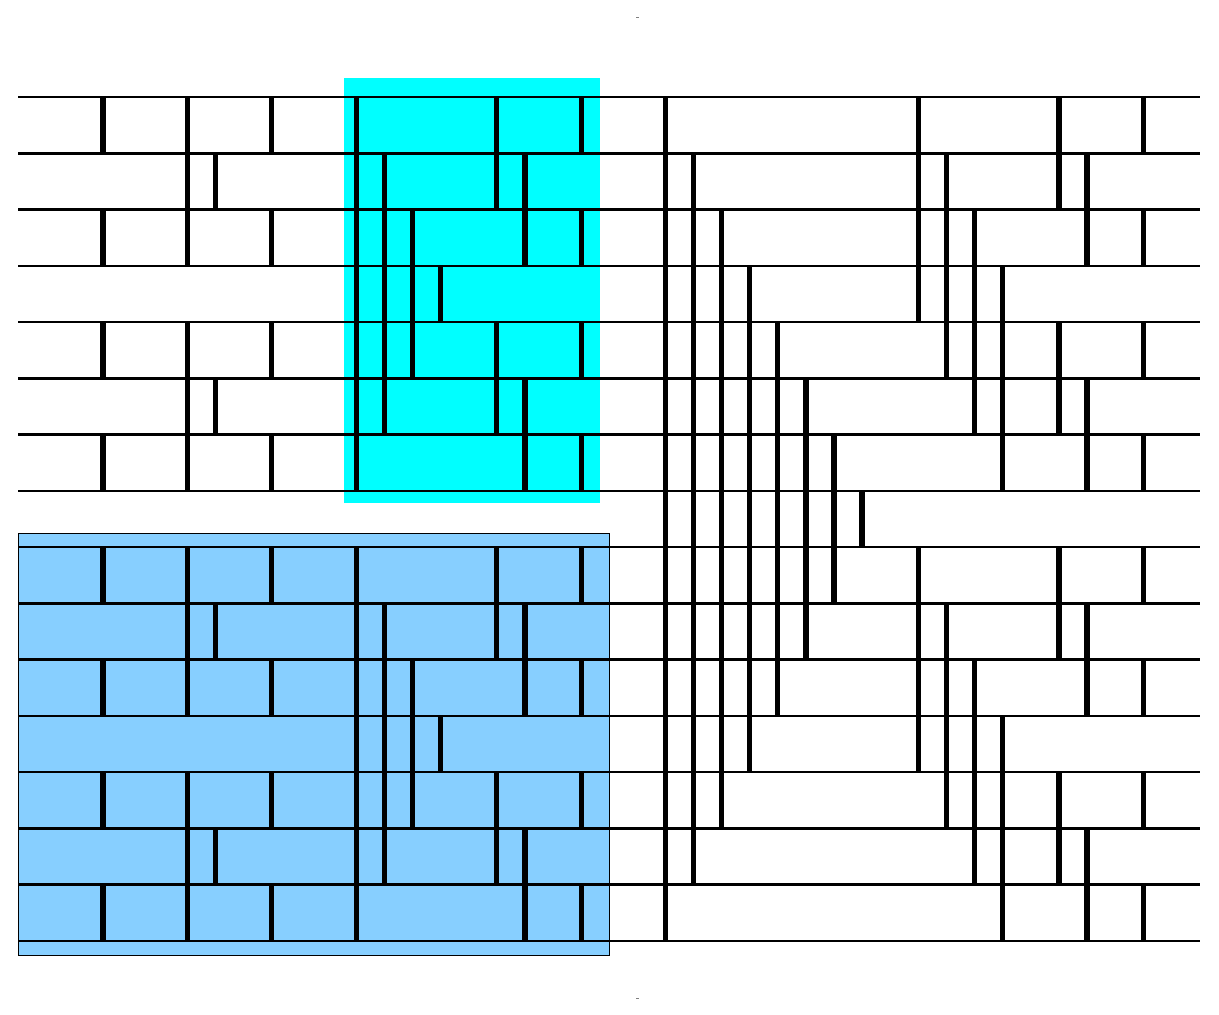
\includegraphics[scale=0.33]{./expressive/mmixedsorter}
\caption{A 16-input sorter made from a tree of {\em tmerge} mergers. 8 2-input mergers
feed 4 4-input mergers, followed  by 2 8-input and one 16-input merger.
A sorter on 8 inputs is shaded, as is a merger on 8 inputs, above it. 
}
\label{fig:mixedsorter}
\end{figure}
\noindent
The following call writes the resulting CUDA to file {\tt tsort1.cu}
and this is the first {\em generated} CUDA kernel whose performance is measured in section~\ref{sec:benchmarks}.

\begin{codesize}
\begin{verbatim}
runs1 k
  = writeFile "tsort1.cu" $ CUDA.genKernel "tsort1" 
      (compose (tsort1 k)) (namedArray "inp" (2^k))
\end{verbatim}
\end{codesize}

The generated code
% for $8$ inputs is shown in Appendix A. It 
uses
one thread per array element (just as the {\tt bitonicMerge}
kernel shown above did). The next step is to move to using Push as
well as Pull arays, so as to be able to generate more efficient code
from essentially the same sorter construction.

\subsection{New combinator implementations using Push arrays}

%% ** TODO make code for ilv2 more comprehensible :)

It is in combining the results of the {\tt f} and {\tt g} functions
that we run into difficulty using just Pull arrays.
Earlier, we saw how to use Push arrays to implement {\tt concP},
which concatenates two arrays.
Here, we use exactly the same approach to make a new version of
the {\em interleave} combinator. The results of applying
the {\tt f}s and {\tt gs} are combined into a Push array, in the right
order.
\pagebreak
%% ** TODO More explanation needed.
\begin{codesize}
\begin{verbatim}
ixMap :: (UWordE -> UWordE) -> ArrayP a -> ArrayP a 
ixMap f (ArrayP p n) = ArrayP (ixMap' f p) n

ixMap' :: (UWordE -> UWordE) 
         -> P (UWordE, a)
         -> P (UWordE, a) 
ixMap' f p = \g -> p (\(i,a) -> g (f i,a))

insertZero :: Int -> UWordE -> UWordE
insertZero 0 a = a `shiftL` 1
insertZero i a 
  = a + (a .&. fromIntegral (complement (oneBits i :: Word32)))

ilv2 :: Choice b => 
        Int -> (a -> a -> b) -> (a -> a -> b) -> 
        Array a -> ArrayP b
ilv2 i f g (Array ixf n) 
   = ArrayP (\k -> app a5 k *>* app a6 k) n
  where
    n2 = n `div` 2
    a1 = Array (ixf . left) (n-n2)
    a2 = Array (ixf . right) n2
    a3 = zipWith f a1 a2
    a4 = zipWith g a1 a2
    a5 = ixMap left (push a3)
    a6 = ixMap right (push a4)
    left = insertZero i
    right = flipBit i  . left
    app (ArrayP f _) a = f a
\end{verbatim}
\end{codesize}
\noindent
This new combinator can now replace {\tt ilv1} in the bitonic
merger, giving a kernel that runs considerably faster. We will use
that kernel to build a large sorter later.

The implemenation of {\tt vee2} is almost identical to
that of {\tt ilv2}, with {\tt flipBit i}
replaced by {\tt flipLSBsTo} as before (so that, again, one would in
fact make a more generic function for building such combinators).
Now, we just need to replace the {\tt ilv1} and {\tt vee1} combinators
in the tree sorter with {\tt ilv2} and {\tt vee2} , to get a verrsion that uses half as many threads:
\begin{codesize}
\begin{verbatim}
tmerge2 :: Int -> [Array IntE -> ArrayP IntE]
tmerge2 n = vstage (n-1) : [ istage (n-i) | i <- [2..n]]
  where
    vstage i = vee2 i min max
    istage i = ilv2 i min max


tsort2 :: Int -> [Array IntE -> ArrayP IntE]
tsort2 n = concat [tmerge2 i | i <- [1..n]]
\end{verbatim}
\end{codesize}
As we shall see in section~\ref{sec:benchmarks}, the resulting code
is significantly faster. This is because it uses one thread per two array elements,
and the code no longer contains any conditionals.

In order to go faster still, we resort to building a different sorting network, of
exactly the same size as the bitonic sorter, but based instead on the balanced period merger of Dowd et al~\cite{PeriodicBalanced}.
This involves the introduction of one new combinator that can be seen as a mixture
of the {\tt ilv} and {\tt vee} combinators already introduced.

\subsection{A sorter built from the balanced periodic merger}
First, we note that the balanced periodic merger contains multiple
uses of the now familiar vee-shaped pattern, see Figure~\ref{fig:periodicMerger}.
\begin{figure}
\centering

\includegraphics[scale=0.25]{./expressive/balanced}
\caption{16 input periodic balanced merging network}
\label{fig:periodicMerger}
\end{figure}

\begin{codesize}
\begin{verbatim}
bpmerge2 :: Int -> [Array IntE -> ArrayP IntE]
bpmerge2 n = [vstage (n-i) | i <- [1..n]]
  where vstage i = vee2 i min max
\end{verbatim}
\end{codesize}

Now Dowd et al proved that the balanced periodic merger sorts two {\em interleaved} sorted sequences. So, taking an iterative view of the resulting sorter,
we want to build a tree of mergers as before, but the smaller mergers should
be interleaved, rather than operating on adjacent sub-sequences.
There should be one merger on the right hand end of the network; left of
that, there should be two mergers that operate on the odd and even elements,
and each of them should in turn be fed by two interleaved mergers, and so.
The sorter is illustrated, for $16$ inputs in Figure~\ref{fig:vsorter}.
Just to the left of the final balanced merger, one of the two interleaved
mergers is shown using dotted lines. It operates on a completely different set of inputs from the other 8-input merger in the same part of the tree.

\begin{figure*}
\centering
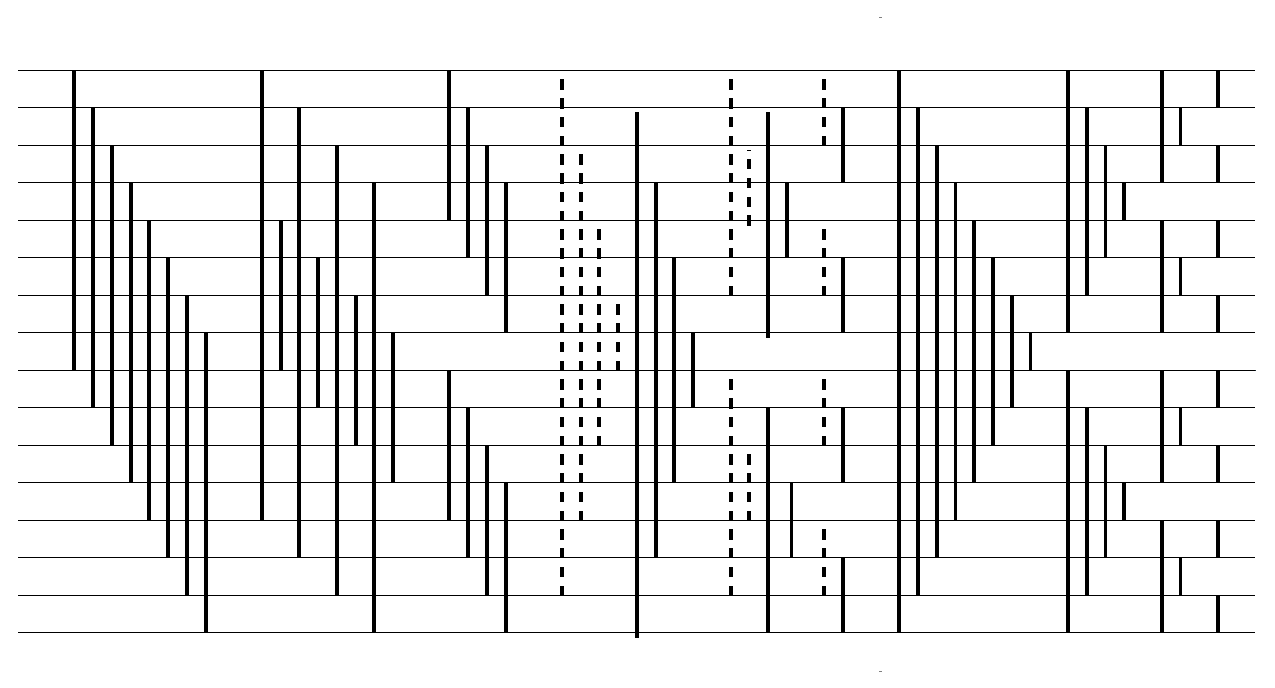
\includegraphics[scale=0.5]{./expressive/vsorter}
\caption{A sorter based on the idea that the periodic
balanced merger network sorts two interleaved sorted sequences.
It consists of two half-sized sorters, one working on the
odd elements of the input and one on the even, followed by
the balanced merger. The diagram indicates using dotted lines the
balanced merger that is the final (rightmost) part of
one of the half-size sorters.}
\label{fig:vsorter}
\end{figure*}

The most straightforward way to give an iterative description of
this sorter is
to introduce a new combinator that is a combination of
{\tt ilv} and {\tt vee}.
The only thing that we need to change is the {\em partner} function.
This time we will flip not the least significant bits from position $0$ to
position $i$ but from position $i$ to $i+j$.

\begin{codesize}
\begin{verbatim}
-- flip bits from position i to position i+j inclusive
flipBitsFrom :: Bits a => Int -> Int -> a -> a
flipBitsFrom i j a = a `xor` (fromIntegral mask)
  where
    mask = (oneBits (j + 1):: Word32) `shiftL` i

ilvVee1 :: Choice a => 
           Int -> Int -> 
           (b -> b-> a) -> (b -> b -> a) -> 
           Array b -> Array a
ilvVee1 i j f g arr = Array ixf (len arr)
  where
    ixf ix = let l = arr ! ix
                 r = arr ! newix
                 newix = flipBitsFrom i j ix
             in (ifThenElse (lowBit (i+j) ix) (f l r) (g l r))
\end{verbatim}
\end{codesize}

\begin{codesize}
\begin{verbatim}
ilvVee2 :: Choice b => Int -> Int -> 
           (a -> a -> b) -> (a -> a -> b) -> 
           Array a -> ArrayP b
ilvVee2 i j f g (Array ixf n) 
  = ArrayP (\k -> app a5 k *>* app a6 k) n
  where
    n2 = n `div` 2
    a1 = Array (ixf . left) (n-n2)
    a2 = Array (ixf . right) n2
    a3 = zipWith f a1 a2
    a4 = zipWith g a1 a2
    a5 = ixMap left (push a3)
    a6 = ixMap right (push a4)
    left = insertZero (i+j)
    right = flipBitsFrom i j . left
    app (ArrayP f _) a = f a
\end{verbatim}
\end{codesize}

For both variants of the combinator, we simply add to the {\tt ilv} definitions
a new {\tt Int} parameter, {\tt j}, and replace {\tt flipBit i} by {\tt flipBitsFrom i j}. We also insert the zero bit (when calculating the left index)
at position {\tt i + j} rather than just at position {\tt i}.
{\tt ilvVee} is a generalisation of both {\tt ilv} and {\tt vee}.
{\tt ilvVee i 0} has the same behaviour as {\tt ilv i}, and {\tt ilvVee 0 (j-1)}
is the same as {\tt vee j}. The {\tt i} parameter controls the degree
of interleaving, and the {\tt j} parameter controls the size of
the vee-shaped blocks.

For $16$ inputs, the parameters
to {\tt ilvVee} that describe the periodic merger on the right of the construction
are $i=0$ (for no interleaving) paired with $3$, $2$, $1$ and $0$
for the decreasing size of the vee-shaped blocks.
Next, to the left, the mergers are interleaved ($i=1$) and there are three
stages with
vee-shaped blocks of decreasing size ($j = 2, 1, 0$), see Figure~\ref{fig:vsorter}.
The following code gives an iterative description of the construction
for {\small $2^n$} inputs:


\begin{codesize}
\begin{verbatim}
vsort :: Int -> Array IntE -> Kernel (Array IntE)
vsort n = composeS . map pure $ [istage (n-i) (i-j) 
                                | i <- [1..n], j <- [1..i]]
  where istage i j = ilvVee2 i j min max
\end{verbatim}
\end{codesize}

\noindent
The resulting generated code uses one thread per
$2$ indices.

\subsection{Measuring performance of the generated kernels}\label{sec:benchmarks}
\begin{figure}
\begin{codesize}
\begin{verbatim}
  unsigned int arrayLength = 1 << LOG_L_SIZE;
  unsigned int diff = LOG_L_SIZE - LOG_S_SIZE;
  unsigned int blocks = arrayLength / S_SIZE;
  unsigned int threads = S_SIZE / 2;
  
  sortSmall<<<blocks, threads,4096>>>(din,din);
 
  for(int i = 0 ; i < diff ; i += 1){ 
    vSwap<<<blocks/2,threads*2,0>>>(din,din,(1<<i)*S_SIZE);
     
    for(int j = i-1; j >= 0; j -= 1)
      iSwap<<<blocks/2,threads*2,0>>>(din,din,(1<<j)*S_SIZE);
      
    bmergeSmall<<<blocks,threads,4096>>>(din,din);}
\end{verbatim}
\end{codesize}
\caption{CUDA code for our large sorter. {\tt sortSmall} and {\tt bmergeSmall}
are replaced by Obsidian-generated kernels in the experiments. {\tt vSwap} and {\tt iSwap} are handwritten CUDA kernels
that perform one column of compare and swap operations in the vee and ilv shapes respectively, and are
parameterised on the stride. (Our generated kernels have fixed input and output size.)}
\label{fig:CUDAsort}
\end{figure}
We have measured the performance of generated 512-input sorting and merging kernels by plugging them into a larger sorter written in CUDA.
The sorter has exactly the structure shown in Figure~\ref{fig:mixedsorter}.
Figure~\ref{fig:newmixedsorter} shows the location of smaller sorters and mergers, and of vSwap and iSwap kernels for $16$ inputs.
Larger sorters simply have more columns of mergers, each preceded by a vSwap and a number of iSwaps.
The overall structure of the resulting CUDA code is shown in Figure~\ref{fig:CUDAsort}.
Because {\tt iSwap} is used repeatedly, we also wrote kernels
corresponding to compositions of two and three of them (avoiding
memory accesses between the columns).
That is, we replaced the loop containing {\tt iSwap} above by
\pagebreak
\begin{codesize}
\begin{verbatim}
for(int j = i-1; j >= 0; j -= 3){ 
  if (j==0) 
    iSwap<<<blocks/2,threads*2,0>>>(din,din,(1<<j)*S_SIZE);
    else 
    {if (j==1) 
       iSwap2<<<blocks/4,threads*2,0>>>(din,din,(1<<j)*S_SIZE);
       else 
       iSwap3<<<blocks/8,threads*2,0>>>(din,din,(1<<j)*S_SIZE);}}
\end{verbatim}
\end{codesize}
\noindent
The Obsidian implementation and all code for examples in the paper are available at \url{http://www.cse.chalmers.se/~joels/expressive.html}.

\begin{figure}
\centering
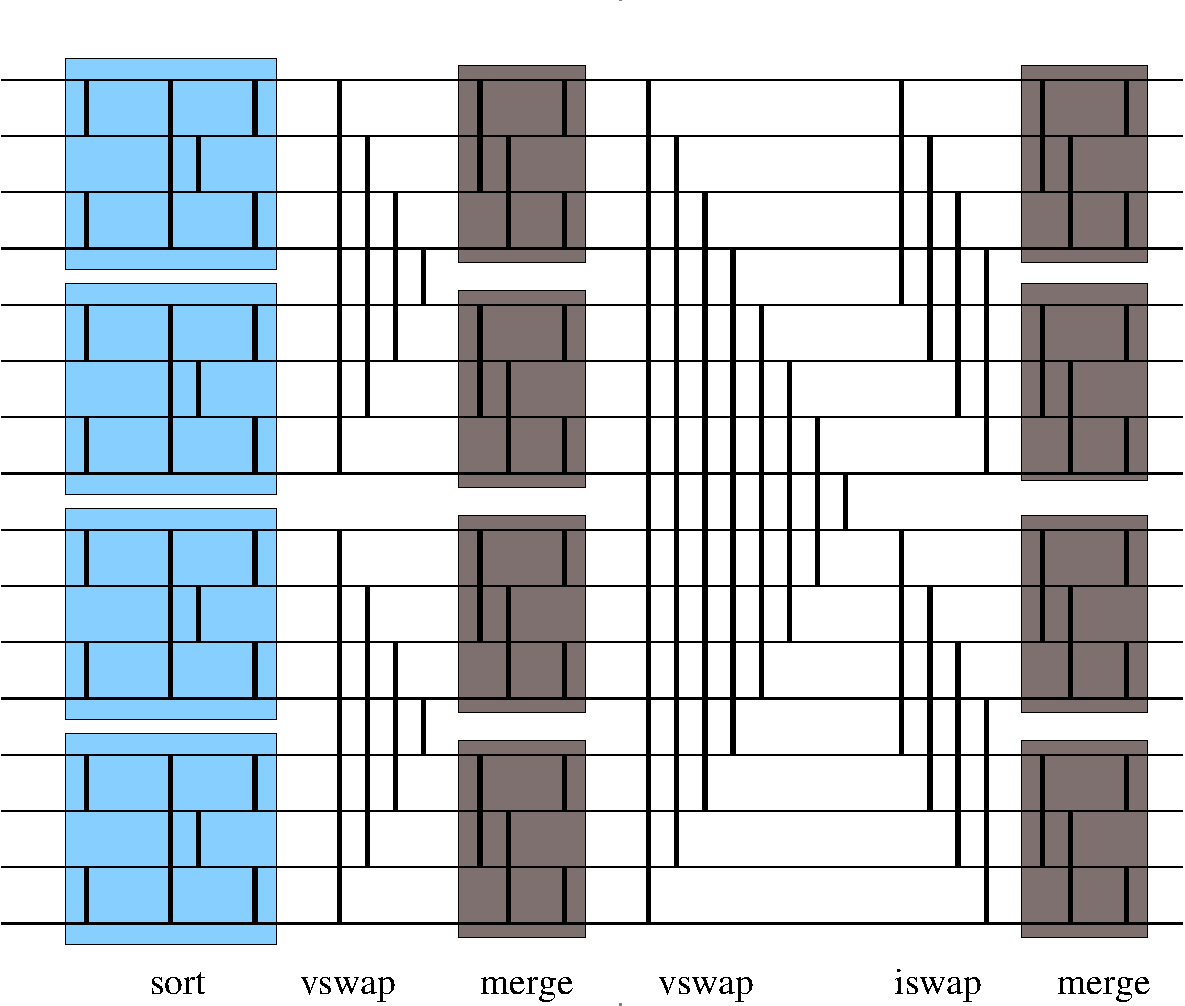
\includegraphics[scale=0.33]{./expressive/newmixedSorter}
\caption{
This diagram shows the tree-shaped sorting network that we saw earlier, but with 4 input sorting and merging kernels indicated. This is the structure of the network that we have used to implement large sorters, in which the small kernels having {\small $2^9 = 512$} inputs in all cases. For {\small $2^{24}$} inputs overall, the resulting sorter
has one column of small sorters and $24-9=15$ of small mergers.}
%% both ofs in the above sentence should remain :)
\label{fig:newmixedsorter}
\end{figure}

Table~\ref{fig:table} shows the performance figures for the large sorter
for $5$ different $512-$input small sorter kernels.
{\tt tsort1} is defined above, and is a variant of bitonic sort
that does not require {\tt if} statements to determine the direction
of sorting of pairs, as all comparison operations place the minimum at the
same index as the lower input.
{\tt tsort2} is the same construction, but built with the combinators {\tt ilv2}
and {\tt vee2} that result in the use of one thread per two indices.
{\tt vsort}, the fastest kernel, uses a generalisation of those
two combinators, and again uses one thread per two indices.
{\tt vsort1} is the same construction as {\tt vsort}, but with {\tt ilvVee2} replaced
by {\tt ilvVee1}, and so using one thread per index.
As a reference small kernel implementation, we include a simple hand-coded bitonic sort
that uses one thread per index (see code in Appendix).
None of the kernels has been subject to optimisations related to warp size.

% table 


\begin{table}
\begin{center}
  \begin{tabular}{| l | r | r | r | r | r | r | }
    \hline
        k                             &  $20$ &  $21$ & $22$& $23$ & $24$ & $24$(CPU)  \\ \hline
    bitonic(CUDA)(512)                &  5 & 12 & 25 & 54 & 117 & 2741   \\      
    tsort1(512)                       &  4 & 10 & 22 & 47 & 102 & 2742    \\
    tsort2(256)                       &  4 & 9 & 23 & 45 & 98 & 2741     \\ 
    vsort1(512)                       &  4 & 10 & 21 & 47 & 102 & 2747    \\ 
    vsort(256)                        &  4 & 9 & 20 & 44 & 96 & 2783    \\ 
    \hline
  \end{tabular}
\end{center}
\label{tab:expressive-table1}
\caption{Sorting time (ms) for $2^k$ inputs, $20 \leq k \leq 24$.  The GPU used is an NVIDIA GTX480.
Each line shows the result using a particular small $512$ input sort kernel with the
indicated number of threads as {\tt sortSmall} in the CUDA code above. The small merge kernel used
is our generated {\tt bmerge2}, with two indices per thread and $512$ inputs. Memory transfer time (GPU-CPU)
is not shown. In the $2^{24}$ input case using {\tt vsort}, the total sorting time, including
memory transfers was 141 ms.
The rightmost column shows the time taken for the C quicksort function {\tt qsort}, compiled with
{\tt gcc -O3}, to sort the same inputs as those sorted on the GPU on an i7-920 2.8GHz CPU.
} 
\end{table}




%% bitonic 30203
%% 


We also recorded the GPU time spent in the calls to the small sorters alone (using the NVIDIA CUDA Visual profiler), see Table~\ref{tab:table2}.
The {\tt tsort1} and {\tt vsort1} kernels, which are built using only pull arrays, 
(and which have one index per thread in the generated code) are
noticeably slower than those that have two indices per thread.
The generation of the latter kernels is made possible by the introduction of 
push arrays.

% table 


\begin{table}
\begin{center}
  \begin{tabular}{| l | r | r |   }

    \hline
                              & time & percent \\ \hline
    bitonic(CUDA)             & 30203 & 32.07\\
    tsort1                    & 15823 & 19.72  \\
    vsort1                       & 14955 & 18.76 \\ 
    tsort2                      & 11562 & 15.37    \\ 
    vsort                       & 9228 &  12.67 \\ 
    bitonic (NVIDIA SDK)        & 23815 & 6.55 \\
    \hline
  \end{tabular}
\end{center}
\label{tab:expressive-table2}
\caption{time: GPU time (in $\mu$s) spent in calls to small sorter kernels 
in the initial phase of the sorter for $2^{24}$ inputs. percent: percentage 
of total GPU time spent in the small sort kernel.
The final line shows the numbers for the bitonic code (for large sorts) that 
is distributed with the the NVIDIA SDK. Its structure also starts with a phase 
of small sorting kernels. It takes 274 ms to sort $2^{24}$ key-value pairs on 
an NVIDIA GTX480 GPU. It could be sped up by using our {\tt vsort} kernel, 
and also by (hand) fusing single ``column'' kernels as we did with {\tt iSwap}, 
although the need to calculate directions of comparators in the bitonic network 
would complicate this. Our CUDA code is simpler because all comparators
point in the same direction in the sorter construction.
} 
\end{table}






%% bitonic 30203
%% tsort1 15823
%% tsort2 11562
%% vsort1 14955
%% vsort 9228


Although none of our generated kernels is optimised (for example with respect to warp size), 
their performance is, nevertheless, very good. We are working on automated warp size-related 
optimisations. It would also be interesting to explore the fusion of adjacent columns of 
comparators in the small kernels; omitting a {\tt sync} would cause this fusion to happen
but we also need to modify the threading behaviour (doubling the number of indices per thread).


%The final version of the paper will contain benchmarking against a highly optimised sorter kernel obtained from our colleagues in the computer graphics group at Chalmers. For now, we emphasise that the {\tt vsort} kernel is so fast that we expect it to compare favourably. Given the simplicity of its description in Obsidian, we feel that this is a good way to write fast kernels.



\section {Discussion}

%% ** TODO. Mention CSE. warp-related opt.

Push arrays form a new approach to array representation in DSELs.
We do not know of similar approaches in the literature, despite
the fact that the notions of demand and data flow
may feel familiar to the reader who considers Pull and Push arrays.
The addition of Push arrays to Obsidian seems highly beneficial. With 
this new feature, the user gains finer grained control over the code generated
and the resulting CUDA kernels perform considerably better than before.
This 
was illustrated in the series of sorters explored in section~\ref{sec:MARY}.
The performance of {\tt vsort} is sufficiently good that it
can be used as a first phase in a larger sorter (written in CUDA) that
can sort 16M elements in 96 ms, while an i7-920 CPU takes
around 2740 ms. Further speed improvements look possible, both in the coordination code
and in the kernels. An obvious next step would be to investigate the generation of the {\tt iSwap} and
{\tt vSwap} kernels from Obsidian. (This is not currently possible because of assumptions that we made about the interfaces to kernels and about how {\em thread ids} are used. We will look into ways to relax
our assumptions.)

The series of kernels also illustrates how the use of combinators brings a form of reuse, and makes design exploration easier. Our experience of using similar combinators in the Lava hardware
description language~\cite{LavaSorter} was that a relatively small set of combinators went a long way. So, although we introduced three
combinators here, {\tt ilv}, {\tt vee} and {\tt ilvVee}, which
includes the other two, we do not believe that every new kernel development exercise would demand a completely new set of combinators.
We expect to provide the user with a well-documented set of combinators,
so that users can get access to this style of programming without having
to develop their own combinators, and without having to think too much
about bit-hacking.
The bit-manipulation approach chosen to define our combinators automatically
created functions that apply to sub-sequences of the input that
are of an appropriate length.

In this paper, we made combinators for the special case of two input, two
output operations (built from two two-input funtions that we typically called
{\tt f} and {\tt g}). 
This approach should be generalised to deal with blocks that have $2^k$ inputs
and outputs.
Also, we made a compound combinator from {\tt ilv} and {\tt vee},
but generalising to more than two input components would allow
for composing combinators, and indeed for recursive descriptions
that could be unrolled. Then, ignoring {\tt syncs}, a recursive description of
{\tt vsort} could be something like 
\begin{codesize}
\begin{verbatim}
vsortR 0 = id
vsortR n = bpmergeR n . ilv2 1 (vsortR (n-1))
\end{verbatim}
\end{codesize}
\noindent
It would then be necessary to optimise the code generated from
multiple applications of {\tt ilv2 1}, for example, whereas here
we have forced the user to figure out both the unrolling and the combinations.
Moving to more general combinators would also give the opportunity to
provide predefined combinators that capture more of the commonly used threading patterns (for instance $k$ indices per thread rather than the $1$ and $2$ shown here).

The integration of Push arrays into Obsidian raises some new questions.
Previously, there was a direct correspondence between the length 
of an array and the number of threads used to compute it, which
allowed the user to write an initial program without worrying about
threads at all, and then to tweak the Obsidian program if he was not satisfied
with the threading behaviour of the resulting kernel. 
Now, as can be seen in the {\tt catArrayPs} example and in the sorters, this correspondence
can be broken using Push arrays. The {\tt catArrayPs} example and two
of the sorters use half as many threads as the 
number of elements. For users who are very concerned about the speed of
the generated kernels, getting this control through using Push arrays in
a particular pattern is clearly a good thing. But adding a second, different
way to control thread use in the generated code certainly complicates matters, and further case studies are needed to confirm that the complication pays off.

The addition of Push arrays also adds the possibility to include potentially 
unsafe operations in Obsidian, for example by writing multiple array elements to the same index, or by discarding elements.
This new expressiveness will have to be carefully controlled. On the positive side, it offers the possibility to encode functions like {\tt filter} from Haskell
that
are simply not expressible using only Pull arrays. Being able to implement {\tt filter} would make programming kernels in obsidian feel much more like programming in Haskell -- a welcome loosening of the strait-jacket.
Once that is done, it will be time to develop a very simple coordination language to allow programming of entire GPU applications that make use of
the kind of small kernel building blocks developed here.





%\appendix
\section{Appendix}
\begin{codesize}
\begin{verbatim}
__device__ inline void swap(int & a, int & b)
{
   int tmp = a;
   a = b;
   b = tmp;
}

__global__ static void bitonicSort(int * values, int *results)
{
   extern __shared__ int shared[];

   const unsigned int tid = threadIdx.x;
   const unsigned int bid = blockIdx.x;

   // Copy input to shared mem.
   shared[tid] = values[(bid*NUM) + tid];

   __syncthreads();

   // Parallel bitonic sort.
   for (unsigned int k = 2; k <= NUM; k *= 2)
   { 
     // bitonic merge
     for (unsigned int j = k / 2; j>0; j /= 2)
       {
           unsigned int ixj = tid ^ j;

           if (ixj > tid)
           {
               if ((tid & k) == 0)
               {
                   if (shared[tid] > shared[ixj])
                   {
                       swap(shared[tid], shared[ixj]);
                   }
               }
               else
               {
                   if (shared[tid] < shared[ixj])
                   {
                       swap(shared[tid], shared[ixj]);
                   }
               }
           }
           __syncthreads();
       }
   }

   // Write result.
   results[(bid*NUM) + tid] = shared[tid];
}
\end{verbatim}
\end{codesize}





\section*{Acknowledgments} 
This research has been funded by the Swedish Foundation for Strategic Research (which funds
the RAW FP Project) and
by the Swedish Research Council.


% We recommend abbrvnat bibliography style.

%\bibliographystyle{abbrvnat}
%\bibliography{paper}

% The bibliography should be embedded for final submission.

%\begin{thebibliography}{}
%\softraggedright

%\bibitem[Smith et~al.(2009)Smith, Jones]{smith02}
%P. Q. Smith, and X. Y. Jones. ...reference text...

%\end{thebibliography}

%\end{document}

